%Please use LuaLaTeX or XeLaTeX
\documentclass[11pt,aspectratio=169]{beamer}

\usepackage[ngerman]{babel}
\usepackage{ragged2e}

\definecolor{ethblue}{RGB}{32, 91, 174}
\definecolor{mygrey}{RGB}{175, 175, 175}

\hypersetup{
  colorlinks=true,
  urlcolor=ethblue,
  linkcolor=ethblue,
  citecolor=ethblue
}

\title{Theoretische Informatik}
% \date[ABC 2021]{24. Sep 2026}
\date[]{8. Okt 2026}
\author{Olivér Kovács}
% \institute{Organizational Unit\\can spread over 2 lines}

\usetheme{eth}

\colorlet{titlefgcolor}{ETHBlue}
\colorlet{accentcolor}{ETHRed}

\begin{document}

%\def\titlefigure{elements/title-page-image}		% Default image
%\def\titlefigure{elements/title-page-image-43}	% Use this for 4:3 presentations

\titleframe

% \tocframe

% \section{Layout}

\begin{frame}{Organisatorisches}
    \begin{itemize}
        \item Nachteilsausgleich
        \begin{itemize}
            \item Email an \href{mailto:hjb@inf.ethz.ch}{hjb@inf.ethz.ch}
        \end{itemize}
    \end{itemize}
\end{frame}

\begin{frame}{Serie Aufgabe 3}
    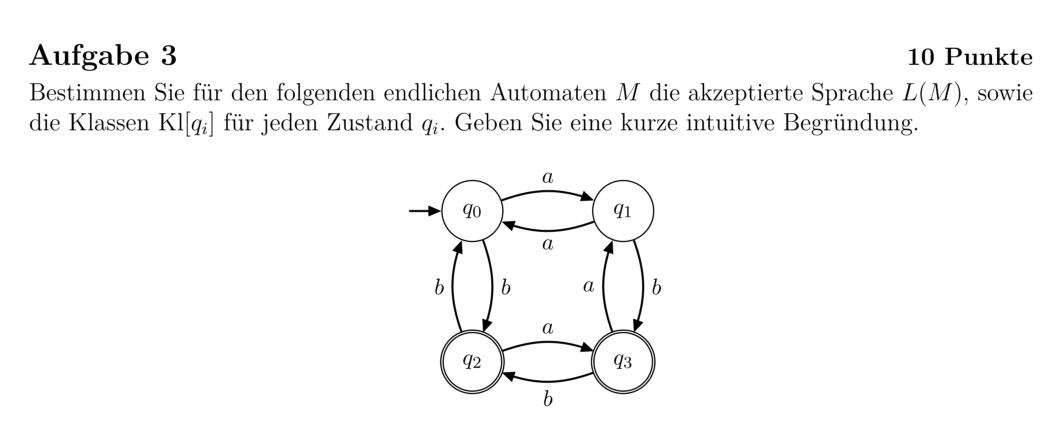
\includegraphics[width=32em]{img/a3}
\end{frame}

\begin{frame}{Serie Aufgabe 4 (b) Musterlösung}
    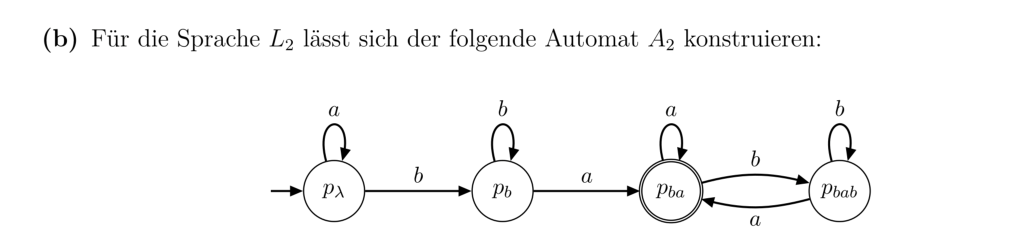
\includegraphics[width=32em]{img/a4b}

    Aber geht es besser?
\end{frame}

\begin{frame}{Wie zeigt man Nichtregularität?}
    \justify
    \textbf{Lemma 3.4. (Pumping-Lemma)}
    Sei \(L\) regulär. Dann existiert eine Konstante \(n_0 \in \mathbb N\),
    so dass sich jedes Wort \(w \in \Sigma^*\) mit \(|w| \ge n_0\) als \(w = yxz\)
    zerlegen lässt, wobei
    \begin{enumerate}
        \item \(|yx| \le n_0\),
        \item \(|x| \ge 1\),
        \item entweder \(\{yx^kz \mid k \in \mathbb N\} \subseteq L\) oder
            \(\{yx^kz \mid k \in \mathbb N\} \cap L = \varnothing\).
    \end{enumerate}

    \vspace{2em}

    Beweis?
\end{frame}

\begin{frame}{Nichtdeterminismus}

\textbf{Definition 3.3.}
Ein \textit{nichtdeterministischer endlicher Automat (NEA)} ist ein
Quintupel \(M = (Q, \Sigma, \delta, q_0, F)\) wobei
\begin{itemize}
    \item \(Q\) eine endliche Menge von \textit{Zuständen} ist,
    \item \(\Sigma\) ein Alphabet \textit{(Eingabealphabet)} ist,
    \item \(\delta \colon Q \times \Sigma \to \mathcal P(Q)\) die \textit{Übergangsfunktion} ist,
    \item \(q_0 \in Q\) der Anfangszustand ist,
    \item \(F \subseteq Q\) die \textit{akzeptierenden} Zustände sind.
\end{itemize}

\end{frame}

\begin{frame}{Nichtdeterminismus}
\textbf{Satz 3.2.} Zu jedem NEA \(M\) existiert ein EA \(A\), so dass \(L(M) = L(A)\).

\vspace{2em}

Beweis?

\end{frame}

% \setbeamertemplate{footline}{}

\begin{frame}{Aufgaben}
    \begin{enumerate}
        \justifying
        \item \textbf{Aufgabe 1.}
            Beweise, dass die Sprache \(L = \{w \in \{0, 1\}^* \mid w = w^R\}\) über \(\{0, 1\}\) nicht regulär ist.
        \item \textbf{Aufgabe 2.}
            In Quiz Frage 3 steht \(L = \{(ababa)^{2n} ab (abaab)^{3n} \mid n \in \mathbb N\}\) sei regulär.
            Konstruiere einen NEA \(M\) mit \(L(M) = L\).
        \item \textbf{Aufgabe 3.}
            Konstruiere einen NEA mit höchstens fünf Zuständen, der
            \[
                L_3 = \{ w \in \{a, b\}^* \mid |w| = 2 \text{ oder } w \text{ endet mit } ab \text{ oder } w \text{ endet mit } ba\}
            \]
            akzeptiert. Begründe die Korrektheit deiner Konstruktion.
        \item \textbf{Aufgabe 4.}
            Konstruiere mittels Potenzmengenkonstruktion einen EA für \(L_3\).
    \end{enumerate}
\end{frame}

\end{document}
